\documentclass[a4paper,12pt,bibliography=totoc,index=totoc,twoside,francais]{scrbook}
%\documentclass[a4paper,12pt,DIVcalc,bibliography=totoc,index=totoc,twoside,francais]{scrbook}
\KOMAoptions{titlepage,chapterprefix,open=right}
%\KOMAoptions{bibliography=totoc,index=totoc}
%\addtokomafont{chapter}{\rmfamily}
%\addtokomafont{section}{\rmfamily}

\usepackage[utf8]{inputenc}
\usepackage[T1]{fontenc}
\usepackage{lmodern}
\usepackage{graphicx}
\usepackage[automark,headsepline]{scrpage2}
\usepackage[style=numeric,sorting=none,backend=biber]{biblatex}
\usepackage{csquotes}
\usepackage{xspace}
\usepackage[autolanguage]{numprint}
\usepackage{array}
\usepackage{booktabs}
\usepackage[table,svgnames,dvipsnames]{xcolor}
\usepackage[final]{pdfpages} 
\clubpenalty=5000
\widowpenalty=5000

%\usepackage{lipsum}

\usepackage{makeidx}
\makeindex
\usepackage[xindy={language=french,codepage=utf8},acronym,toc=true,nonumberlist]{glossaries}
\makeglossaries
\newacronym{sdn}{SDN}{Software-Defined Networking, Réseau Informatique Défini par Logiciel}
\newacronym{rtfm}{RTFM}{Read the f\dots manual}

\usepackage[english,francais]{babel}
\frenchbsetup{og=«, fg=»}
%\bibliography{biblio}

\usepackage[backend=biber]{biblatex}
\addbibresource{biblio.bib}

\usepackage[pdfauthor={Cynthia Lopes do Sacramento}, pdftitle={SDN : Software-Defined Networking}]{hyperref}

\pagestyle{scrheadings}

\begin{document}
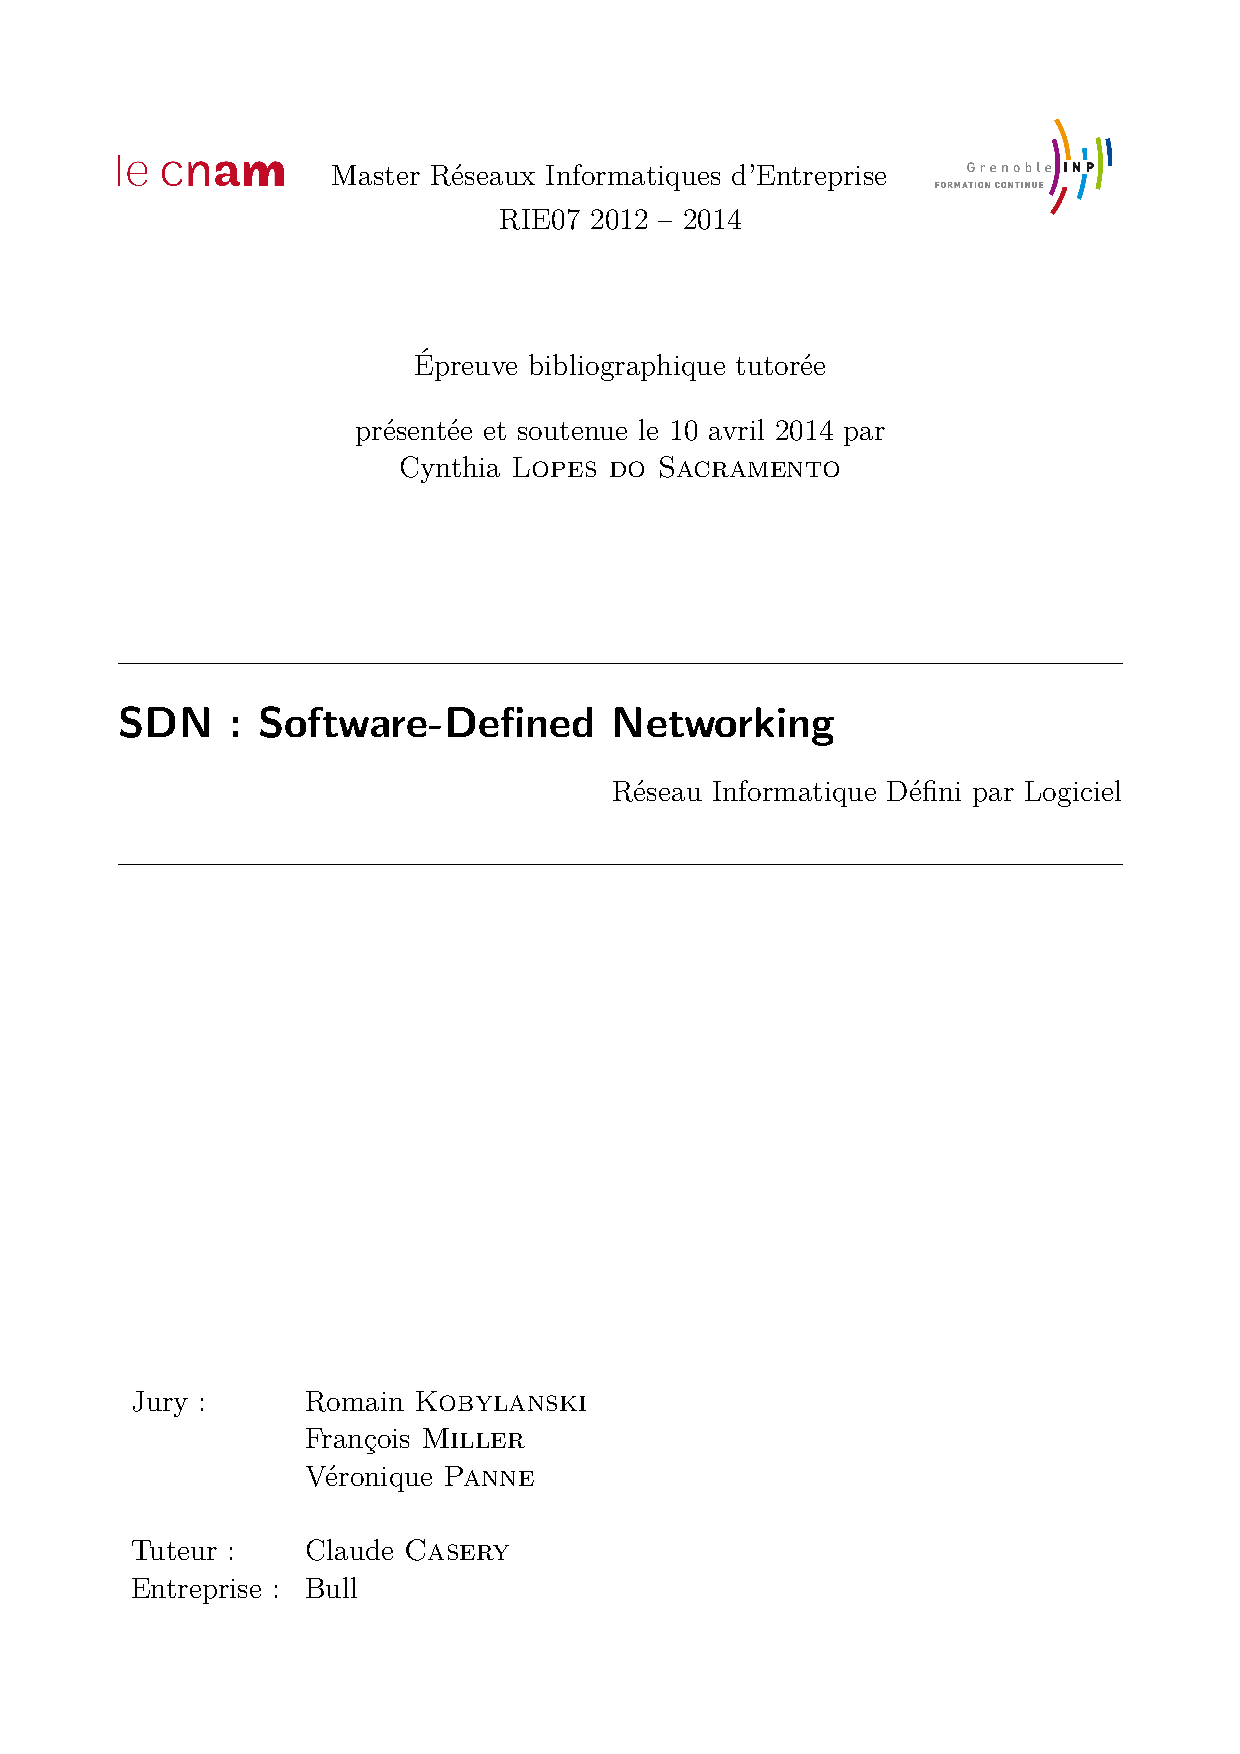
\includepdf[pages={1-2}]{couverture-ebt.pdf}

\frontmatter
\begin{flushright}
Chaque fois que les gens découvrent son mensonge,\\
Le châtiment lui vient, par la colère accru.\\
« Je suis cuit, je suis cuit ! » gémit-il comme en songe.\\
~\\
Le menteur n'est jamais cru.\\
\end{flushright}

\tableofcontents
\listoftables
\listoffigures

\mainmatter
%\addchap{Introduction}
\addchap{Introduction}

%\section{To Do}
%Parler de la croissance (de l'explosion même) de l'utilisation de l'internet. Du hypertexte aux applications dynamiques. Puis la virtualisation et le cloud computing. Ensuite le big data. Montrer que ça évolue en grande vitesse.
%\par Expliquer que l'architecture et l'infrastructure réseau n'avaient pas été conçues pour ce scénario. Donc ça commence à se saturer ne correspondant plus aux besoins actuels. Les choses sont plus éphémères, il y a besoin de quelque chose plus flexible, adaptable. Et l'architecture actuelle pose des difficultés pour l'expérimentation des nouveaux protocoles, services, applications etc. 
%\par Introduire SDN comme une réponse à cette problématique. Expliquer brièvement ce que c'est et pour quoi cela apporte une évolution. Montrer comment ça pourrait être utilisé pour répondre aux besoins actuels.
%\par Expliquer les objectifs du texte : ré-définir SDN, présenter les enjeux et les cas d'utilisation et un état de l'art des technologies qui sont sorties.
%\par Présenter la méthodologie, le développement du texte et de quoi va parler chaque section. 
 

%\section{Évolution de l'utilisation Internet pendant une décade}

[3 lignes qui parlent de SDN et utilisent les mots clefs du sujet.]

L'internet a évolué de trois manières importantes dans les dix dernières années. 
\begin{itemize}
\item Le contenu a évolué de texte et pages web relativement statiques, il a progressé vers un contenu multimédia haut-débit exigeant une latence réduite. 
\item L'utilisation s'est rapidement mondialisée; par exemple le débit international servant l'Afrique a augmenté de 1.21Gbit/s en 2001 à 570.92Gbit/s en 2011 \cite{InternetGlobalGrowthImpactDevelopingCountries}.
\item  L'accès a étendu des ordinateurs de bureau à une variété de nouveaux dispositifs, comme pour les téléphones mobiles dont le trafic global des donnés a augmenté de 70\% en 2012. \cite{CiscoVNI2013}. 
\end{itemize}
Fait important: la rapidité d'une telle évolution technologique et son adoption est sans précédent dans l'histoire de l'humanité. 


\par
La capacité d'évolution pour s'adapter aux nouvelles exigences des usagers est recourrente dans l'histoire de l'Internet. 
%La croissance accélérée de l'accès de partout, notamment dans les pays en développement et la rapide augmentation de l'utilisation par les utilisateurs existants, dirigées par les contenus multimédias et application machine-à-machine sont des 
En revanche, dans le scénario actuel on voit poindre une croissance accélérée de l'accès de partout, notamment dans les pays en développement, ainsi qu'une rapide augmentation de l'utilisation par les utilisateurs existants, engendrée par les contenus multimédias et les applications machine-à-machine. Par exemple, en moins de deux ans depuis la parution d'Instagram, plus de 50 millions de personnes on partagé plus d'un milliard de photos desssus. \cite{deuxAnsInstagram}.
Dans ce contexte, on met en cause capacité de l'internet, comme il est, de continuer à fournir l'infrastructure nécessaire. \cite{InternetSustainGrowthIntro}
\par
De nouvelles technologies et concepts émergent pour répondre aux nouveaux besoins de ces utilisateurs qui exigent de plus en plus haut-débit et une latence réduite. Le \gls{bigdata} a modifié le traitement des données pour permettre les entreprises de gérer la quantité massive de données manipulées. \cite{IMBigData} Le \gls{cloudcomputing} et la \gls{virtualisation} ont apporté une nouvelle approche pour le management et l'hébergement de ressources de \gls{ti} dans le but de les rendre plus agiles, plus efficaces, plus sécurisés et plus flexibles tout en réduisant les coûts. \cite{CloudComputingIntelVision}. Pour accompagner ces évolutions, une innovation technologique dans le domaine des réseaux informatiques est requise. \cite{InternetEvolutionRoleSoftwareEngineeringConclusion}
\par
Cette problématique a amené scientifiques et tout les ingénieurs impliqués dans ce secteur à la conception de \gls{sdn}. \gls{sdn} est un nouveau \glslink{paradigme}{paradigme} réseau qui est actuellement développé en collaboration pour adapter l'infrastructure existante au nouveau scénario.\cite{OpenFlowStanford} Le présent document a donc pour but d'explorer cette solution et analyser les approches qui ont été faites dans ce domaine. Il propose un état de l'art des technologies parues pour déployer \gls{sdn} ainsi que divers cas d'utilisation dont les enjeux seront présentés.
\par
[un paragraphe pour le plan du texte (de quoi parle chaque section)]
\par
[Un paragraphe pour conclure l'intro et laisser les pistes de mon point de vue et les conclusions trouvées].




\chapter{Problématique Réseau et SDN}
\label{chap-1}

%\section{Première section}\label{sec-1-1}

%\section{Deuxième section}\label{sec-1-2}

%Ce chapitre va reprendre les problèmes réseaux rencontrés pour définir les besoins actuels dans le domaine. Une liste de requis pour une architecture réseau idéalement adapté aux applications actuelles sera proposée.
%En connaissant les problèmes de l'architecture en place, la question que se pose est : si on repartait de zéro, comment on le ferrait ?

%\section{Pression pour l'expansion de l'architecture réseau }

\section{Ossification de l'internet face au besoin d'expansion}



%"The classic Internet architecture is a victim of its own success. Having succeeded so well at empowering users and encouraging innovation, it has been made obsolete by explosive growth in users, traffic, applications, and threats." The range of problems observed today is not surprising.

%The Internet was created in simpler times, among a small club of cooperating stakeholders. As the Internet becomes part of more and more aspects of society, it will inevitably be subject to more demands from more stakeholders, and be found deficient in more ways

%In the first half of the 2000s, the research climate was dominated by the belief that research is pointless unless its results can be adopted easily within the existing Internet. Attempting to work within this constraint, people realized that the current architecture makes solving some problems impossible.


À vouloir autoriser et même encourager les utilisateurs à innover sur son architecture, l'internet s'est fait dépasser par son propre succès. La croissance explosive des utilisateurs, du trafic et des applications a apporté toute une série de problèmes, 
%L'internet a été créé à une époque où les choses étaient plus simples, avec peu d'intervenants en coopération. Dès qu'il est devenu partie intégrante en plusieurs aspects de la société, diverses réclamations et défaillances sont apparues, 
tant que l'exhaustion des adresses IPv4 disponibles et les menaces aux réseaux locaux privés. 

%One of the main reasons for these security vulnerabilities is that the Internet architecture and its supporting protocols were primarily designed for a benign and trustworthy environment, with little or no consideration for security issues. This assumption is clearly no longer valid for today’s Internet, which connects millions of people, computers, and corporations in a complex web that spans the entire globe.
\par
En réponse à ces questions, on a introduit dans l'architecture des \glspl{middlebox}, par exemple les NATs et les Firewalls, à un prix : la complexité. Le logiciel dans ces systèmes est capable d'atteindre n'importe quel objectif sous réserve de devenir excessivement complexe, fragile, incompréhensible et mal jugé. Parce que les coûts de la complexité ont été négligés lors de l'évolution de l'internet, les applications en réseau sortantes ont été rendues difficiles à concevoir, à mettre en place et à maintenir. \cite{InternetEvolutionRoleSoftwareEngineeringRealInternet}

Actuellement l'internet compte avec une énorme base d'équipements et de protocoles installée. Avec le système d'adressage IPv4 ce réseau peut interconnecter jusqu'à quatre milliards d'équipements. Capacité dont le limite est proche d'être atteint, confirmé par le développement du protocole IPv6 qui nous permettrait d'augmenter l'espace d'adressage par des centaines de milliards de fois. \cite{ICANNIPv6Important} 

L'internet est vu aujourd'hui comme une infrastructure critique de la société, tel que le transport ou l'électricité.  Cela provoque une résistance aux essais des nouvelles applications en parallèle à celles en mode de production. 
Ce fait a mené la communauté de chercheurs en réseau à se faire dominée par une conviction de qu'un travail n'est utile que si ses résultats peuvent être facilement adoptés dans l'architecture existante. En essayant de travailler avec cette contrainte, les concepteurs ont réalisé que l'architecture courante rend la résolution de certains problèmes impossible. \cite{OpenFlowStanfordOssification} \cite{SurveySDNIntro}

%illustrer les problèmes, donner un apperçu



%Complexity matters. The trouble with software is that it can do anything, no matter how complex, convoluted, fragile, incomprehensible, and ill-judged. Software engineers understand the cost of such complexity. Because the networking community underestimates the cost of complexity, it pays no attention to one of the most important problems of the current Internet, which is that it is much too difficult to build, deploy, and maintain networked applications.

%From the viewpoint of Internet users and application programmers, there are requirements that sometimes equal or exceed performance, availability, and efficiency in priority. These include ease of use, correctness, predictability, and modularity.

%The routing table in a typical router now has 300,000 entries, and these must be stored in the fastest, most expensive types of memory to maintain routing speed.

On se rend compte que l'adoption de nouvelles idées dans le domaine des réseaux reste complexe.  Finalement, les ingénieurs comptent avec peu de moyen concret pour tester de nouveaux protocoles réseau dans une configuration assez réaliste pour assurer et distribuer leurs déploiements. Par conséquent, la majorité des nouvelles idées émises dans le cadre de la recherche en "réseaux informatiques" finissent sans essais et sans tests. Cette barrière à l'évolution en face des besoins d'expansion des utilisateurs actuels confirme la croyance répandue que l'infrastructure réseau "est en phase d'ossification". \cite{OpenFlowStanfordOssification} 

%quantifier enorme.

\section{Management Réseau : Pénible et Complexe}

%\subsection*{Brain storming *}

%Même dans un réseau LAN de porte moyen,  on compte avec plusieurs équipements qui réalisent des fonctions spécifiques. Ces équipement doivent être configurable un à un donc pour atteindre à un objectif pour le réseau, tous la configuration de chaque équipement doit être orchestrée pour aboutir ce besoin. Il est difficile de mettre un place une configuration centralisée.

%\par Chaque équipement a été conçu pour réaliser une fonctionnalité spécifique. Pour toute correction de bug ou extension de ces fonctions,  il est nécessaire que le vendeur mette en place une mis à jour logiciel tenant en compte les modifications souhaités ou alors il faut acheter un nouveau équipement. 

%\par Difficulté de faire évoluer (lack of scalability or inability to scale) ; Complexité générant une résistance à l'innovation ; Dépendance du vendeur ; politiques inconsistantes

%Even with the help of autonomous and intelligent agents and network management software, the job of a network administrator is important and complicated. They must balance the different network management areas to make sure their system is properly configured and maintained. 

%The Internet was not designed with management in mind, yet the administrators of today’s networks face critical problems of configuration, traffic engineering, routing policy, and failure diagnosis. Their tools for understanding network traf- fic are poor, and their mechanisms for controlling network operations do not offer a predictable relationship between cause and effect.

%Internet routing is beginning to have serious problems of scale. The routing table in a typical router now has 300,000 entries, and these must be stored in the fastest, most expensive types of memory to maintain routing speed.2 There are efforts to move toward a scheme in which a typical routing table has one entry per autonomous system, which points to a router that can route to all the addresses for which that autonomous system is responsible.

%Network configuration and installation requires highly-skilled personnel adept at configuration of many network elements. Where interactions between network nodes (e.g. switches, routers, etc.) are complex, a more systems-based approach encompassing elements of simulation is required. With the current programming interfaces on much of today’s networking equipment, this is difficult to achieve. In addition, operational costs involved in provisioning and managing large, multi-vendor networks covering multiple technologies have been increasing over recent years, whilst the pre- dominant trend in revenue for operations has been decreasing.

%It was noted that network operation and management is a major source of operating costs, and as well a source of failures and disruptions due to operator error. So we can expect major changes in this area, and we can expect this to be a major focus of a future architecture design.


%Perhaps the attributes most critically lacking are those relating to security, including highly resilient and dependable availability, and a trustworthy environment for people (and their computers) to communicate.

%\subsection*{Fin brain storming *}

Cette résistance empêchant l'innovation est contradictoire à la rapide croissance de l'internet qui impose une expansion de l'architecture réseau. 
Le besoin pour des services réseau et pour haut-débit augmente à un taux plus rapide que la disponibilité ou les revenues.



\begin{figure}[!h] %on ouvre l'environnement figure
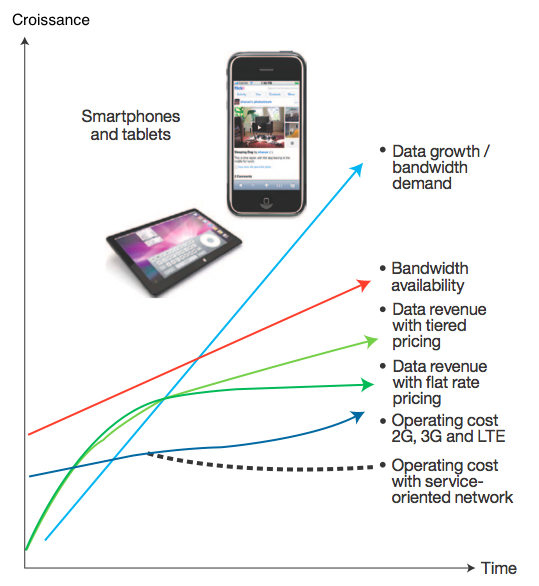
\includegraphics[width=15cm]{images/IncreasingPressureOnNetworkInfra.png} %ou image.png, .jpeg etc.
\caption{ Pression croissante sur l'infrastructure réseau \cite{IBMManagingGrowingPainsNeed}} %la légende
\label{image_soleil} %l'étiquette pour faire référence à cette image
\end{figure} %on ferme l'environnement figure


% Figure 1: The need for network capabilities and bandwidth is expanding at a faster rate than either bandwidth availability or revenue to grow

\clearpage

Le plus une entreprise dépend d'un nombre croissant de dispositifs et gros volumes de données, les plus importante est la demande pour débit et expansion de l'infrastructure. La complexité de cette expansion des réseaux augmente la probabilité des interruptions de service dues à une faille humaine ou autre problème. Ce fait met en évidence l'importance de la disponibilité, fiabilité, performance et sécurité. L'efficacité et la réduction des coûts deviennent cruciales pour aboutir la mis en échelle de ces besoins, et donc le management assume en rôle primordial dans ce contexte. \cite{IBMManagingGrowingPainsNeed}
 

Malgré l'assistance des agents autonomes et intelligents ainsi que des logiciels pour le management réseau, la mission de l'administrateur réseau reste importante et compliquée. Il doit équilibrer les différentes tâches du management pour assurer que le \gls{si} soit proprement configuré et maintenu. \cite{CentralIssuesNetworkManagementConclusion}

La configuration et l'installation du réseau exigent des techniciens experts hautement qualifiés sur plusieurs éléments le composant. Les interactions entre les nœuds du réseau (switches, routeurs etc.) sont complexes, ce qui provoque le besoin pour une approche système englobant la simulation. Avec l'interface de programmation courante des équipements réseau d'aujourd'hui, cela est difficile d'atteindre. De plus, les coûts opérationnels impliqués à l'approvisionnement et management de réseaux larges et multi-vendeurs  couvrant plusieurs technologies ont augmenté récemment, alors que les revenues se diminuent. \cite{ImplementationChallengesForSDN}

L'architecture réseau n'a pas été conçue pour le management, pourtant les administrateurs des réseaux d'aujourd'hui rencontrent des problèmes critiques de configuration, ingénierie du trafic, politique de routage et diagnostic de failles. Leurs outils pour analyse du trafic sont faibles et leurs mécanismes pour contrôler les opérations réseau ne facilitent pas la prédictibilité entre les relations de cause-effet. On réalise que l'opération et le management du réseau représentent la source la plus importante des coûts opérationnels, de failles et d'interruptions à cause d'erreurs des opérateurs. Un changement dans ce domaine est requis pour le design de l'architecture. \cite{NGSIManagement}

%Yet at the same time, society is daring the Internet to face the following set of challenges:
%Security: The lack of security in the Internet is worrisome to ev- eryone including users, application developers, and network and service operators.
%Mobility: Currently, application developers find little support for new mobile applications and services.
%Reliabilityandavailability: ISPsfacethetaskofprovidingaser- vice which meets user expectations of the Internet’s crucial role in both business and private life, in terms of reliability, resilience, and availability, when compared, for example, to the telephone network (five nines1). Furthermore, the service has to be seamless.
%Problem analysis: The toolset for debugging the Internet is lim- ited, e. g., tools for root cause analysis.
%Scalability: Questions remain regarding the scalability of some parts of the current Internet architecture, e.g., the routing system.
%Quality of Service: It is still unclear how and where to integrate different levels of quality of service into the architecture.
%Economics: Besides these more technical questions, there is also the question of how network and service operators can con- tinue to make a profit.



%A new network model is required to support this.
\section{Un nouveau modèle réseau pour supporter ces évolutions}
%\section{Clean-slate Internet}

%While the overall architecture is an undeniable success, the state of the networking industry and the nature of networking infrastructure is a less inspiring story. It is widely agreed that current networks are too expensive, too complicated to manage, too prone to vendor-lockin, and too hard to change. Moreover, this unfortunate state-of-affairs has remained true for well over a decade. Thus, while much of the research community has been focusing on “clean-slate” designs of the overall Internet architecture, a more pressing set of problems remain in the design of the underlying network infrastructure. That is, in addition to worrying about the global Internet protocols, the research community should also devote effort to how one could improve the infrastructure over which these protocols are deployed.

Même si globalement l'architecture réseau d'internet est un succès incontestable, l'état de l'industrie réseau et l'essence de son infrastructure est moins inspirant. Il est partout accepté que les réseaux courants sont excessivement chers, compliqués à gérer, sujets aux blocages des fournisseurs et difficiles à évoluer. En plus, cette condition a bien durée plus d'une décade. \cite{fabricIntro}



En résumé, l'infrastructure réseau confronte actuellement ces challenges:
\begin{itemize}
\item Sécurité : la manque de sécurité est assez inquiétante à tout niveau : des utilisateurs, aux développeurs aux opérateurs de services.
\item Mobilité : il existe très peu de support aux applications et services mobiles
\item Fiabilité et disponibilité : le nouvel usage de l'internet exige de plus en plus haute fiabilité et disponibilité.
\item Analyse de problèmes : les outils pour déboguer les failles réseau sont assez limités.
\item Évolution : certaine partis de l'architecture courante semblent être saturés, comme le système de routage.
\item Qualité de service : il est toujours incertain comment intégrer différents niveaux de qualité de service.
\item Économique : en outre de tous questions techniques, il reste aussi la question de comment les opérateurs pourront continuer à tirer profit.
\end{itemize}
\cite{InernetCleanSlateDesignIntro}

%In the past 30 years the Internet has been very successful using an incremental approach. However due to its success, the commu- nity has now reached a point where people are unwilling or unable to experiment on the current architecture. Therefore, it might be time to explore a clean-slate approach
Dans les dernières 30 années, internet a été bien succédé à utiliser une approche incrémentielle pour répondre aux divers challenges rencontrés. Cependant, grâce à ce succès, la communauté a récemment atteint un point où les personnes sont peu disposées ou incapables d'expérimenter sur cette architecture.  Pour cette raison, il est peut être le moment de d'explorer une nouvelle approche. \cite{InernetCleanSlateDesignApproach}

%Re-partir de zéro. En le faisant, quels sont les caractéristique de l'architecture ?


Cette problématique a amené scientistes et les ingénieurs impliqués à concevoir \gls{sdn}. \gls{sdn} est un nouveau \glslink{paradigme}{paradigme} réseau qu'on fait actuellement en cours de développer pour adapter l'infrastructure existante au nouveau scénario.


%\section{Les requis d'un réseau idéalement adapté aux besoins courants}
\chapter{Réseaux programmables avec SDN}

On cherche à concevoir une architecture plus adaptée aux enjeux de la communication de l'actualité discutés dans le chapitre 1. Cette problématique a amené scientistes et les ingénieurs impliqués à concevoir \gls{sdn}. \gls{sdn} est un nouveau \glslink{paradigme}{paradigme} réseau qu'on est actuellement en cours de développer pour adapter l'infrastructure existante à ce nouveau scénario.
Le but de ce chapitre est de (re)définir SDN et de présenter en quoi SDN répond aux besoins explicités dans le chapitre 1.
%Ce chapitre répond aux questions : Qu'est-ce que SDN ? Qu'est-ce que cela propose ?
Le chapitre propose aussi un point sur la situation de SDN, en présentant les organisations qui l'adopte et ce qui a été développé en terme de standards et protocoles.

\section{Séparation de l'intelligence (contrôle) de la commutation (flux de données)}

%Having recognized the problem, the networking commu- nity is hard at work developing programmable networks, such as GENI [1] a proposed nationwide research facility for experimenting with new network architectures and dis- tributed systems. These programmable networks call for programmable switches and routers that (using virtualiza- tion) can process packets for multiple isolated experimen- tal networks simultaneously.
Ayant adressé cette problématique, la communauté réseau fait beaucoup d'efforts pour le développement des réseaux programmables. Ces réseaux programmables utilisent des switches et des routeurs programmables qui peuvent traiter des paquets pour des multiples réseaux expérimentaux  à la fois, grâce à la \gls{virtualisation}. \cite{OpenFlowStanfordOssification} Divers projets pour les réseaux programmables, comme NETCONF \cite{NETCONF}, Ethane \cite{Ethane}, GENI \cite{GENI} etc. ont été réalisés et en ont servi de base pour ce paradigme qu'on développe et supporte aujourd'hui : \gls{sdn}. 

%SDN is described in this article with the Open Networking Foundation (ONF) [1] definition: “In the SDN architecture, the control and data planes are decoupled, network intelli- gence and state are logically centralized, and the underlying network infrastructure is abstracted from the applications.”

SDN est défini au long de cette étude  selon \gls{onf} : Dans l'architecture SDN, les plans de contrôle et de données sont découpés, l'intelligence et l'état du réseau sont logiquement centralisés, et l'infrastructure du réseau est donc abstraite des applications. \cite{SDNNewNormONFExecutiveSummary}


%The control plane is responsible for configuration of the node and programming the paths that will be used for data flows. Once these paths have been determined they are pushed down to the data plane. Data forwarding at the hardware level is based on this control information.

Le \gls{controlplane} est responsable pour la configuration d'un nœud et pour la programmation des chemins qui seront utilisés par les flux de données. Le \gls{dataplane} fourni au hardware les informations nécessaires à la commutation. \cite{ImplementationChallengesForSDNBackground}



Dans l'architecture réseau traditionnellement déployée, chaque équipement actif contient un plan de contrôle et un plan de données à l'intérieur du même matériel. L'ossification d'internet discuté dans le chapitre 1 est largement attribuée à ce fort couplage entre les deux plans provocant que toutes les décisions sur les flux de donnés soient embarquées dans chaque élément réseau. La manque d'une interface de contrôle commune à tous les dispositifs complique toute évolution que cela soit un simple changement de configuration ou le développement d'une nouvelle application. \cite{SurveySDNArchi}



%As mentioned previously, the so-called Internet “ossifica- tion” [2] is largely attributed to the tight coupling between the data– and control planes which means that decisions about data flowing through the network are made on-board each network element. In this type of environment, the deployment of new network applications or functionality is decidedly non- trivial, as they would need to be implemented directly into the infrastructure. Even straightforward tasks such as config- uration or policy enforcement may require a good amount of effort due to the lack of a common control interface to the various network devices.

Avec SDN, on propose la séparation de ces deux éléments. Le \gls{controlplane} est implémenté par un contrôleur centralisé est commun à tous les équipements qui passent à contenir seulement le \glspl{dataplane} un plus d'un module de communication.  La séparation de la fonction de commutation de la logique de contrôle permet un déploiement plus facile de nouveaux protocoles et applications. La virtualisation et le management du réseau deviennent plus simples et les nombreux \glspl{middlebox} sont consolidés dans le logiciel de contrôle. \cite{SurveySDNArchi} \cite{SDNNewNormONFExecutiveSummary}
%the separation of the forwarding hardware from the control logic allows easier deployment of new protocols and applications, straightforward network visualization and management, and consolidation of various middleboxes into software control.

Dans l'image ci-dessous on voit un schéma illustrant l'ensemble de l'architecture dans les deux cas.

%\begin{figure}[!h] %on ouvre l'environnement figure
%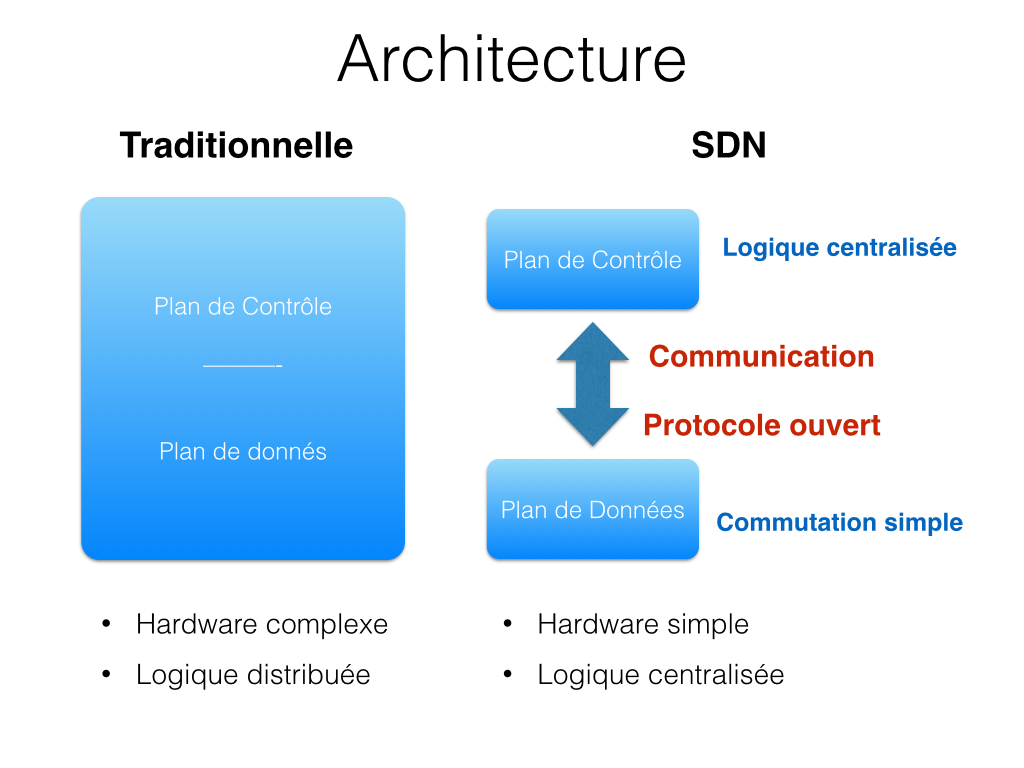
\includegraphics[width=15cm]{images/ComparaisonArchis.png} %ou image.png, .jpeg etc.
%\caption{ Un équipement actif dans l'Architecture Traditionnelle et SDN} %la légende
%\label{imgNodesArchi} %l'étiquette pour faire référence à cette image
%\end{figure} %on ferme l'environnement figure



\begin{figure}[!h] %on ouvre l'environnement figure
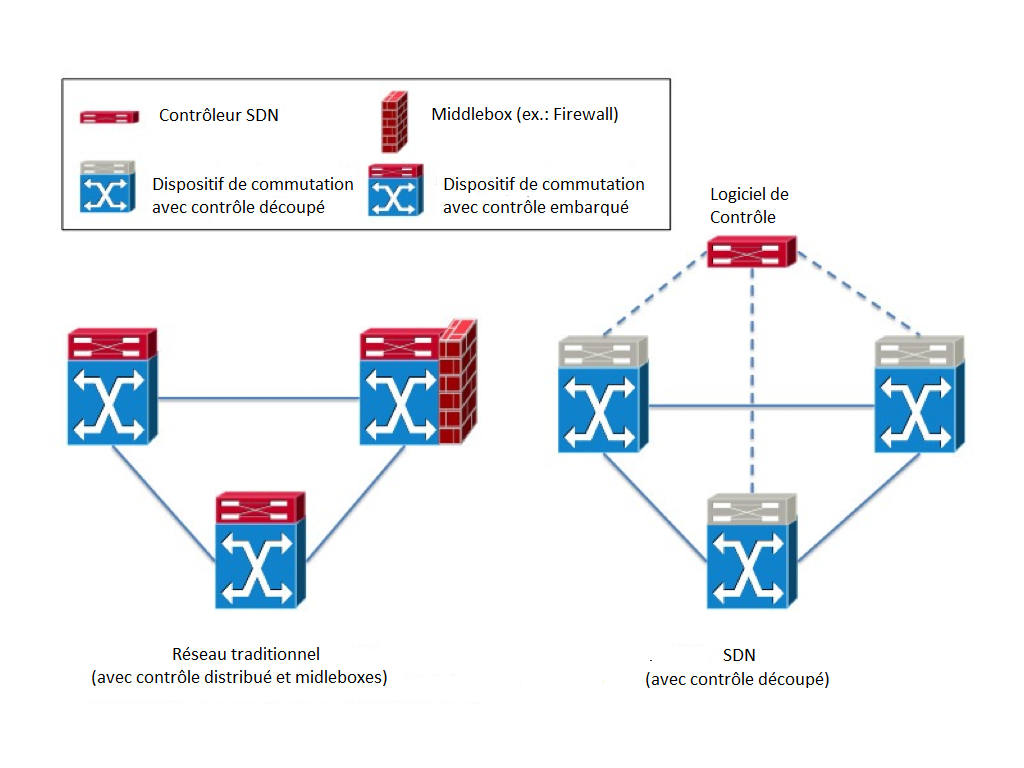
\includegraphics[width=15cm]{images/TraditionalVsSDN.png} %ou image.png, .jpeg etc.
\caption{ L'ensemble de l'Architecture Traditionnelle et SDN \cite{SurveySDNArchi}} %la légende
\label{imgOverviewArchi} %l'étiquette pour faire référence à cette image
\end{figure} %on ferme l'environnement figure

Avec l'approche \gls{sdn} les switchees sont contrôles par un \gls{nos} qui fourni un modèle abstrait de la topologie du réseau au contrôleur \gls{sdn} hébergeant les applications. Le contrôleur peut donc exploiter cet vue globale du réseau pour optimiser le management des flux et supporter les requis de 'scalabilité' et de flexibilité.

%From these service-focussed requirements, SDN has emerged. Control is moved out of the individual network nodes and into the separate, centralized controller. SDN switches are con- trolled by a Network Operating System (NOS) that collects information using the API shown in Figure 2B and manipulates their forwarding plane, providing an abstract model of the network topology to the SDN controller hosting the applications.

\clearpage



\section{Un point sur la situation}
%\subsection{ONF}

%The Open Networking Foundation (ONF) is a non‑profit, user‑driven organization dedicated to accelerating the adoption of open Software‑Defined Networking (SDN). We view SDN as a disruptive approach to networking that will change how virtually every company with a network operates.

%Launched in 2011 by Deutsche Telekom, Facebook, Google, Microsoft, Verizon, and Yahoo!, ONF is a nonprofit organization dedicated to rethinking networking, and quickly and collaboratively bringing to market SDN standards and solutions. ONF is accelerating the delivery and commercialization of SDN and fostering a vibrant market of products, services, applications, customers, and users. 


Open Networking Foudation (\gls{onf}) et une organisation non-profit et axée sur l'utilisateur dédiée à l'accélération de l'adoption ouverte de SDN. Cette organisation voit SDN comme une approche réseau qui va changer comment opère chaque entreprise avec un réseau.
\gls{onf} a été initiée en 2011 par Deutsche Telekom, Facebook, Google, Microsoft, Verizon et Yahoo! dans le but de repenser en collaboration les réseaux informatiques et rapidement apporter au marché les solutions et les standards SDN. Avec la collaboration de  grands experts mondiaux, ONF accélère la commercialisation de SDN en favorisant un vif marché de produits, services, applications, clients et utilisateurs. ONF compte aujourd'hui avec plus de 100 entreprises membres collaboratives de tout taille et variété. \cite{ONFOverview}

\gls{onf} a fait des efforts de standardiser le protocole \gls{openflow}. Ce protocole focalise en standardiser les interfaces entre les applications et le contrôleur et les interfaces entre le contrôleur et l'équipement de commutation.\cite{SurveySDNArchi}
%The Open Network Foundation (ONF) [3] has been trying to standardize the OpenFlow protocol. As the control plane abstracts network applications from underlying hardware infrastructure, they focus on standardizing the inter- faces between: (1) network applications and the controller (i.e. northbound interface) and (2) the controller and the switching infrastructure (i.e., southbound interface) which defines the OpenFlow protocol itself. 

Le fort support de l'industrie, de la recherche et des académies que \gls{onf} et la proposition de \gls{sdn} ont pu recueillir est assez expressif. Les résultats dans ces différents secteurs ont produit un nombre significatif de livrables dans la forme d'articles de recherche, d'implémentations de logiciels de référence et même de hardware. Il y a eu également des efforts de standardisation de SDN de la part d'autres organisations produisant des normes, comme IETF et IRTF. \cite{SurveySDNIntro}
%The strong support from industry, research, and academia that the Open Networking Foundation (ONF) and its SDN proposal, OpenFlow, has been able to gather is quite impres- sive. The resulting critical mass from these different sectors has produced a significant number of deliverables in the form of research papers, reference software implementations, and even hardware. So much so that some argue that OpenFlow’s SDN architecture is the current SDN de-facto standard. In line with this trend, the remainder of this section focuses on OpenFlow’s SDN model. 

%On the academic side, the OpenFlow Network Research Center [4] has been created with a focus on SDN research. There have also been standardization efforts on SDN at the IETF and IRTF and other standards producing organizations.


%\subsection{OpenFlow - Protocoles standardisés}
%\section{Dispositifs de commutation}
%The basic idea is simple: we exploit the fact that most modern Ethernet switches and routers contain flow-tables (typically built from TCAMs) that run at line-rate to im- plement firewalls, NAT, QoS, and to collect statistics. While each vendor’s flow-table is different, we’ve identified an in- teresting common set of functions that run in many switches and routers. OpenFlow exploits this common set of func- tions.

SDN profite du fait que la majorité des switches et routeurs existants contiennent des tableaux de flux qui exécutent à une fréquence ligne pour implémenter leurs protocoles et collecter des statistiques.



%\section{Contrôleur}
Controllers. A controller adds and removes flow-entries from the Flow Table on behalf of experiments. For example, a static controller might be a simple application running on a PC to statically establish flows to interconnect a set of test computers for the duration of an experiment. In this case the flows resemble VLANs in current networks— providing a simple mechanism to isolate experimental traffic from the production network. Viewed this way, OpenFlow is a generalization of VLANs.


\chapter{Enjeux de SDN}

Ce chapitre présente quels sont les enjeux pour déployer SDN. Il a pour but d'identifier les challenges lors de la mise en place de cette architecture ainsi que les problèmes susceptibles d'être rencontrés. Pour chaque enjeux, les idées pour les surmonter sont montrées tout en proposant les compromis de ces solutions.

\section{Contrôle : centralisé ou distribué}
Contrôle centralisé = un seul point de faille pour le réseau complet.

Architecture physiquement distribuée mais centralisé au niveau logique.

Consistence et stateliness quand on distribue des états sur le réseau peut causer un mal comportement des applications qui pensent qu'elles une vision précise du réseau.

\section{Niveau de granularité}

\section{Politiques : réactives ou pro-actives}

\section{Fonctions de Virtualisation du Réseau}
%\gls{nfv}

\addchap{Conclusion}

Même avec le succès incontestable de l'architecture d'internet, l'état de l'industrie réseau et l'essence de son infrastructure se retrouvent en phase critique. Il est généralement admis que les réseaux courants sont excessivement chers, compliqués à gérer, sujets aux blocages des fournisseurs et difficiles à faire évoluer. 

En effet, on constate un réel besoin de faire évoluer cette architecture mais aussi des résistances contraignant cette évolution dues à la complexité et la possible saturation du système. En réponse, les réseaux programmables ont été objet intensif de recherche par la communauté. Les travaux dans le domaine ont progressé vers la proposition de SDN, un nouveau paradigme transformant cette architecture.

L'approche SDN découpe le plan de contrôle et le plan données, offrant un contrôle et une vision centralisés du réseau. Cela peut apporter certains bénéfices comme le contrôle directement programmable, la simplification du hardware réseau et la simplification de l'ingénierie du trafic. En revanche, des challenges d'implémentation sont à surmonter tels que la concentration des risques dans un contrôle physiquement centralisé, l'équilibre entre flexibilité et performance et les conditions d'interopérabilité.

La flexibilité apportée par SDN est telle que de nombreuses possibilités d'applications sont à imaginer. Essentiellement le management de data centers, le contrôle d'accès et de la mobilité pour les réseaux campus ainsi que  l'ingénierie du trafic pour les réseaux WAN.

Le marché suit de près les nouveautés dans le domaine et investit sur les technologies implémentant SDN. Les stratégies sont pas encore assez matures et les potentiels consommateurs attendent des offres plus consolidées. Cependant, des solutions innovantes commencent à surgir et certaines organisations assument un rôle de tête dans le marché.

On s'aperçoit que l'ampleur des possibilités SDN même si un avantage en théorie, frein son adoption. Dû à la massive variété des concepts et produits, les consommateur hésitent toujours à prendre des décisions. Au même temps, les grands fournisseurs cherchent à la fois à exploiter le nouveau marché et à protéger leurs solutions consolidées. Cet impasse même si confirmé, ne semble pas être assez fort pour empêcher les échanges à long terme.

En caractère personnel, cette étude conclue qu'au futur proche, les clients les plus informés et les plus prêt à innover vont commencer à déployer SDN. Vu que leurs expériences et résultats peuvent fortement impacter les choix des prochains consommateurs, il est possible que les premiers à se lancer seront ceux qui vont peindre le futur de la technologie des réseaux informatiques pour les prochaines années. Cette démarche peut représenter un risque au cas échéant, mais aussi l'opportunité d'en tirer des bénéfices plus durables et de prendre de parts plus larges du marché.

\appendix
\chapter{Première annexe}


%\include{ann2}
\gls{rtfm}

\backmatter
\nocite{*}
\printbibliography
\printindex

%\printglossary[type=\acronymtype]
\printglossaries

\cleardoublepage
\includepdf[pages={3-4}]{couverture-ebt.pdf}
\end{document}
